\documentclass{whiteboard}
\begin{document}
\begin{frame}[plain,t]
\bbcover{Programação Lógica}{Backtracking}{Prof. Edson Alves}{Campus UnB Gama: Faculdade de Ciências e Tecnologias em Engenharia}

\end{frame}
\begin{frame}[plain,t]
\begin{tikzpicture}
\node[draw,opacity=0] at (0, 0) {x};
\node[draw,opacity=0] at (14, 8) {x};

	\node[anchor=west] (title) at (0.0, 7.0) { \Large \bbbold{\textit{Backtracking}} };

\end{tikzpicture}
\end{frame}
\begin{frame}[plain,t]
\begin{tikzpicture}
\node[draw,opacity=0] at (0, 0) {x};
\node[draw,opacity=0] at (14, 8) {x};

	\node[anchor=west] (title) at (0.0, 7.0) { \Large \bbbold{\textit{Backtracking}} };


	\node[anchor=west] (a) at (1.0, 6.0) { $\star$ \bbtext{Quando Prolog tenta satisfazer um objetivo a respeito de um predicado, ele percorre} };

	\node[anchor=west] (a1) at (0.5, 5.5) { \bbtext{todas as cláusulas que definem o predicado} };

\end{tikzpicture}
\end{frame}
\begin{frame}[plain,t]
\begin{tikzpicture}
\node[draw,opacity=0] at (0, 0) {x};
\node[draw,opacity=0] at (14, 8) {x};

	\node[anchor=west] (title) at (0.0, 7.0) { \Large \bbbold{\textit{Backtracking}} };


	\node[anchor=west] (a) at (1.0, 6.0) { $\star$ \bbtext{Quando Prolog tenta satisfazer um objetivo a respeito de um predicado, ele percorre} };

	\node[anchor=west] (a1) at (0.5, 5.5) { \bbtext{todas as cláusulas que definem o predicado} };

	\node[anchor=west] (b) at (1.0, 4.5) { $\star$ \bbtext{Se o objetivo e a cláusula unificam, ela satisfaz o objetivo e é marcada} };

\end{tikzpicture}
\end{frame}
\begin{frame}[plain,t]
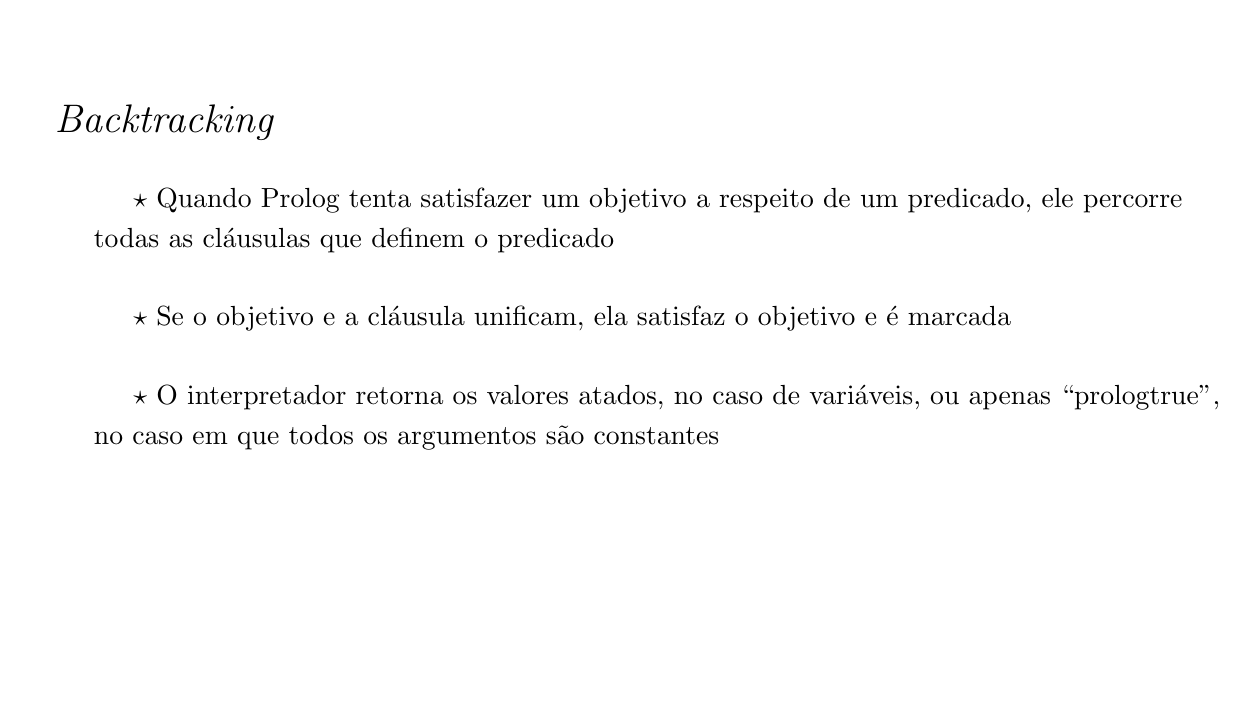
\begin{tikzpicture}
\node[draw,opacity=0] at (0, 0) {x};
\node[draw,opacity=0] at (14, 8) {x};

	\node[anchor=west] (title) at (0.0, 7.0) { \Large \bbbold{\textit{Backtracking}} };


	\node[anchor=west] (a) at (1.0, 6.0) { $\star$ \bbtext{Quando Prolog tenta satisfazer um objetivo a respeito de um predicado, ele percorre} };

	\node[anchor=west] (a1) at (0.5, 5.5) { \bbtext{todas as cláusulas que definem o predicado} };

	\node[anchor=west] (b) at (1.0, 4.5) { $\star$ \bbtext{Se o objetivo e a cláusula unificam, ela satisfaz o objetivo e é marcada} };

	\node[anchor=west] (c) at (1.0, 3.5) { $\star$ \bbtext{O interpretador retorna os valores atados, no caso de variáveis, ou apenas ``\code{prolog}{true}''}, };

	\node[anchor=west] (c1) at (0.5, 3.0) { \bbtext{no caso em que todos os argumentos são constantes} };

\end{tikzpicture}
\end{frame}
\begin{frame}[plain,t]
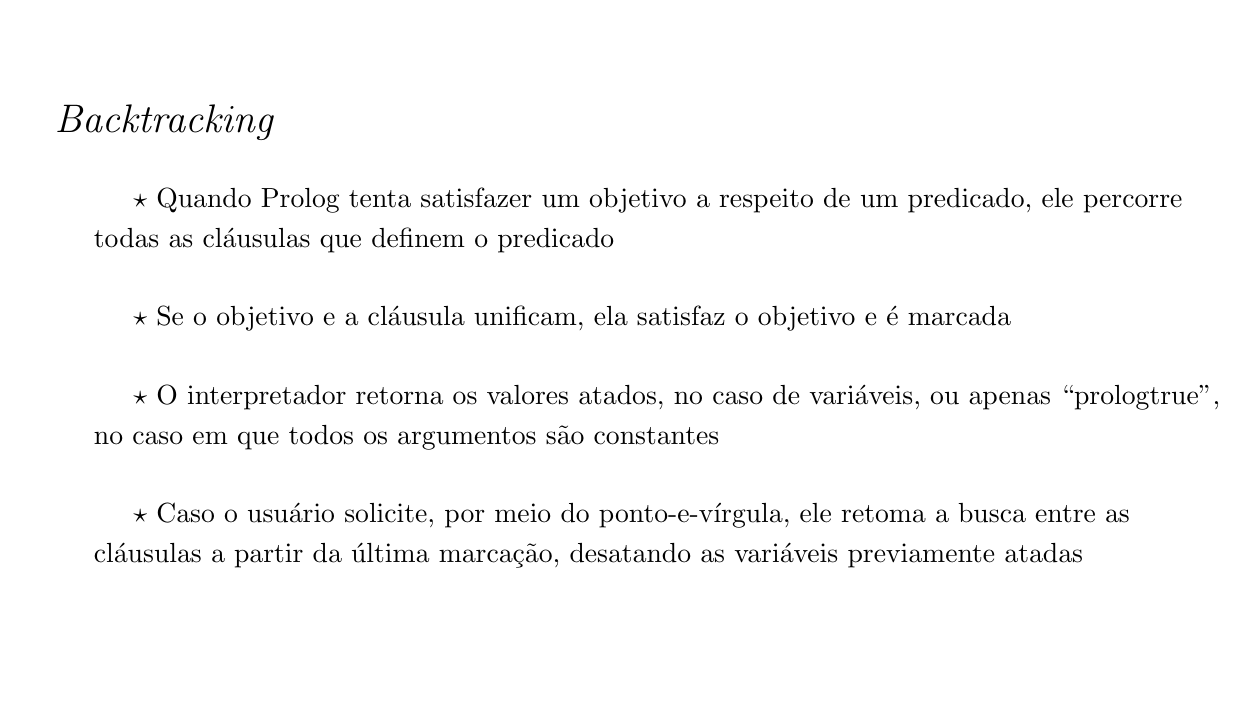
\begin{tikzpicture}
\node[draw,opacity=0] at (0, 0) {x};
\node[draw,opacity=0] at (14, 8) {x};

	\node[anchor=west] (title) at (0.0, 7.0) { \Large \bbbold{\textit{Backtracking}} };


	\node[anchor=west] (a) at (1.0, 6.0) { $\star$ \bbtext{Quando Prolog tenta satisfazer um objetivo a respeito de um predicado, ele percorre} };

	\node[anchor=west] (a1) at (0.5, 5.5) { \bbtext{todas as cláusulas que definem o predicado} };

	\node[anchor=west] (b) at (1.0, 4.5) { $\star$ \bbtext{Se o objetivo e a cláusula unificam, ela satisfaz o objetivo e é marcada} };

	\node[anchor=west] (c) at (1.0, 3.5) { $\star$ \bbtext{O interpretador retorna os valores atados, no caso de variáveis, ou apenas ``\code{prolog}{true}''}, };

	\node[anchor=west] (c1) at (0.5, 3.0) { \bbtext{no caso em que todos os argumentos são constantes} };

	\node[anchor=west] (d) at (1.0, 2.0) { $\star$ \bbtext{Caso o usuário solicite, por meio do ponto-e-vírgula, ele retoma a busca entre as} };

	\node[anchor=west] (d1) at (0.5, 1.5) { \bbtext{cláusulas a partir da última marcação, desatando as variáveis previamente atadas} };

\end{tikzpicture}
\end{frame}
\begin{frame}[plain,t]
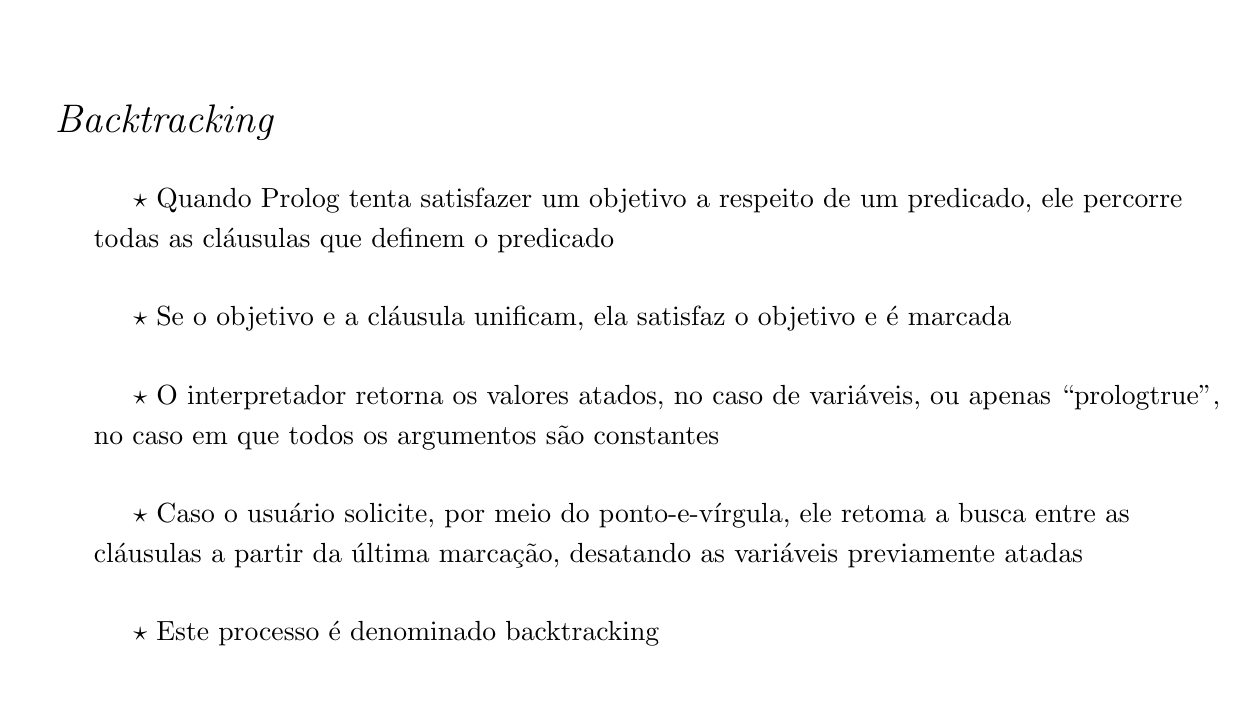
\begin{tikzpicture}
\node[draw,opacity=0] at (0, 0) {x};
\node[draw,opacity=0] at (14, 8) {x};

	\node[anchor=west] (title) at (0.0, 7.0) { \Large \bbbold{\textit{Backtracking}} };


	\node[anchor=west] (a) at (1.0, 6.0) { $\star$ \bbtext{Quando Prolog tenta satisfazer um objetivo a respeito de um predicado, ele percorre} };

	\node[anchor=west] (a1) at (0.5, 5.5) { \bbtext{todas as cláusulas que definem o predicado} };

	\node[anchor=west] (b) at (1.0, 4.5) { $\star$ \bbtext{Se o objetivo e a cláusula unificam, ela satisfaz o objetivo e é marcada} };

	\node[anchor=west] (c) at (1.0, 3.5) { $\star$ \bbtext{O interpretador retorna os valores atados, no caso de variáveis, ou apenas ``\code{prolog}{true}''}, };

	\node[anchor=west] (c1) at (0.5, 3.0) { \bbtext{no caso em que todos os argumentos são constantes} };

	\node[anchor=west] (d) at (1.0, 2.0) { $\star$ \bbtext{Caso o usuário solicite, por meio do ponto-e-vírgula, ele retoma a busca entre as} };

	\node[anchor=west] (d1) at (0.5, 1.5) { \bbtext{cláusulas a partir da última marcação, desatando as variáveis previamente atadas} };

	\node[anchor=west] (e) at (1.0, 0.5) { $\star$ \bbtext{Este processo é denominado \bbenglish{backtracking}} };

\end{tikzpicture}
\end{frame}
\begin{frame}[plain,t]
\begin{tikzpicture}
\node[draw,opacity=0] at (0, 0) {x};
\node[draw,opacity=0] at (14, 8) {x};

	\node[anchor=west] (title) at (0.0, 7.0) { \Large \bbbold{Objetivos e fluxo de controle} };

\end{tikzpicture}
\end{frame}
\begin{frame}[plain,t]
\begin{tikzpicture}
\node[draw,opacity=0] at (0, 0) {x};
\node[draw,opacity=0] at (14, 8) {x};

	\node[anchor=west] (title) at (0.0, 7.0) { \Large \bbbold{Objetivos e fluxo de controle} };


	\node[anchor=west] (a) at (1.0, 6.0) { $\star$ \bbtext{Um objetivo em Prolog tem quatro portas que representam o fluxo de controle de} };

	\node[anchor=west] (a1) at (0.5, 5.5) { \bbtext{sua avaliação: chamada (\bbenglish{call}), saída (\bbenglish{exit}), retomada (\bbenglish{redo}) e falha (\bbenglish{fail})} };

\end{tikzpicture}
\end{frame}
\begin{frame}[plain,t]
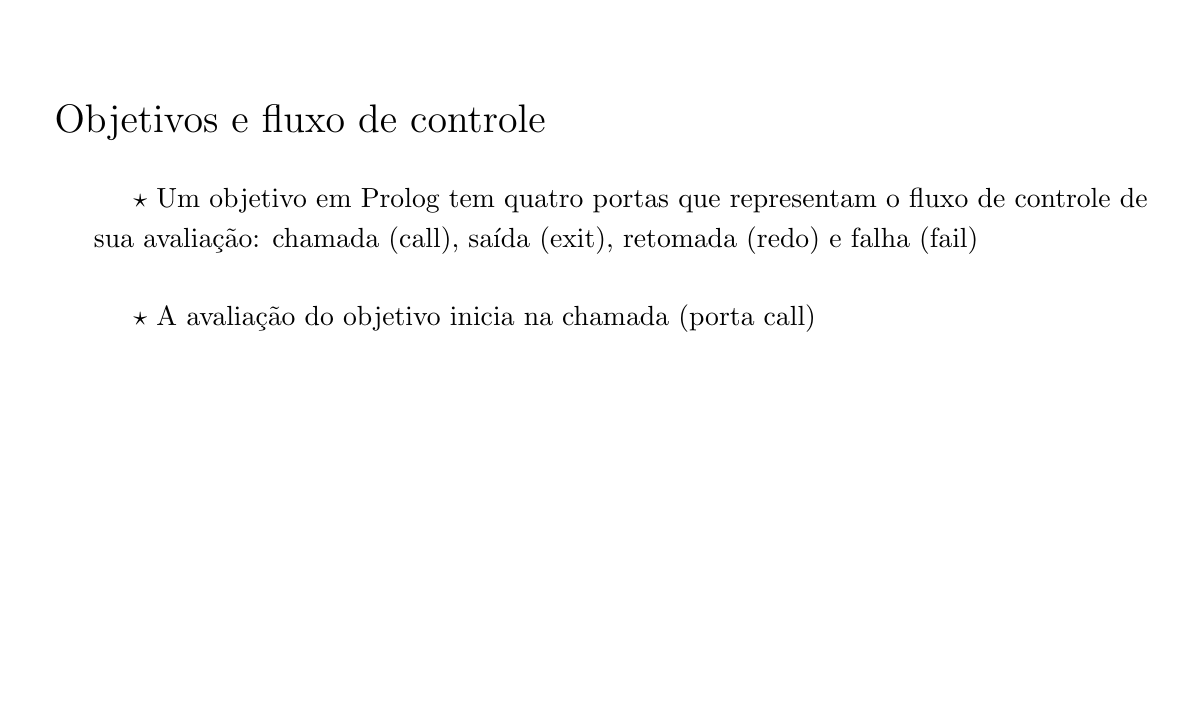
\begin{tikzpicture}
\node[draw,opacity=0] at (0, 0) {x};
\node[draw,opacity=0] at (14, 8) {x};

	\node[anchor=west] (title) at (0.0, 7.0) { \Large \bbbold{Objetivos e fluxo de controle} };


	\node[anchor=west] (a) at (1.0, 6.0) { $\star$ \bbtext{Um objetivo em Prolog tem quatro portas que representam o fluxo de controle de} };

	\node[anchor=west] (a1) at (0.5, 5.5) { \bbtext{sua avaliação: chamada (\bbenglish{call}), saída (\bbenglish{exit}), retomada (\bbenglish{redo}) e falha (\bbenglish{fail})} };


	\node[anchor=west] (b) at (1.0, 4.5) { $\star$ \bbtext{A avaliação do objetivo inicia na chamada (porta \bbenglish{call})} };

\end{tikzpicture}
\end{frame}
\begin{frame}[plain,t]
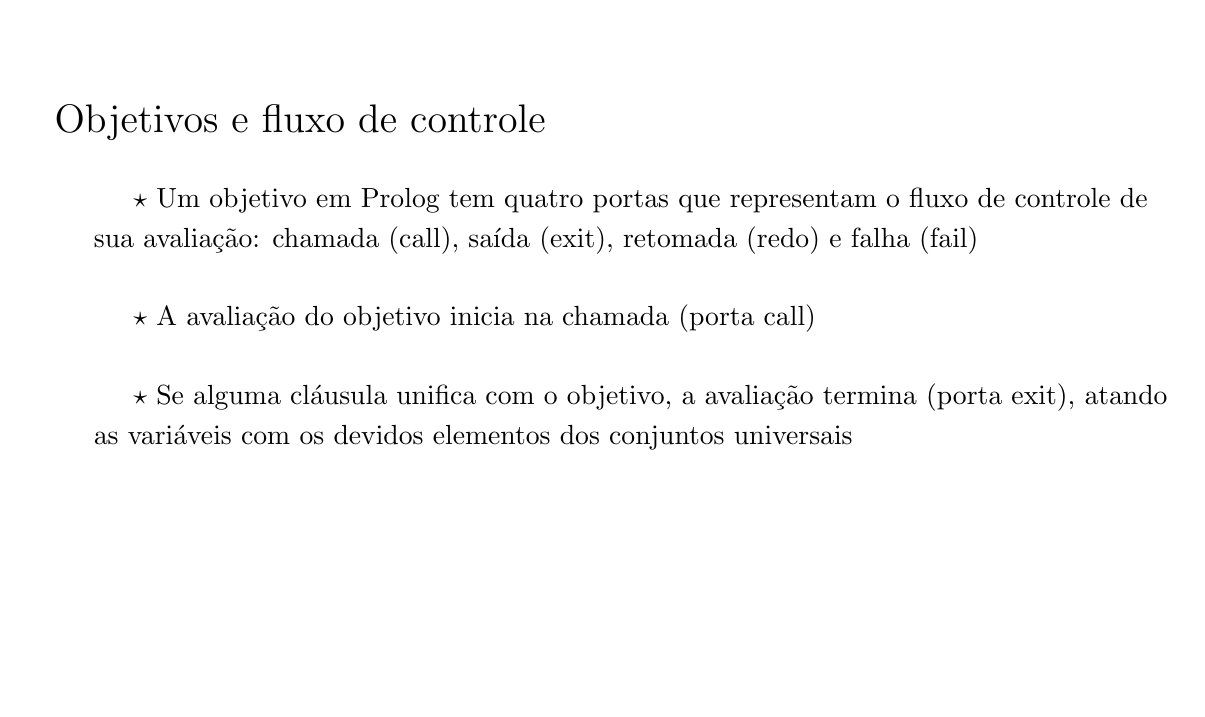
\begin{tikzpicture}
\node[draw,opacity=0] at (0, 0) {x};
\node[draw,opacity=0] at (14, 8) {x};

	\node[anchor=west] (title) at (0.0, 7.0) { \Large \bbbold{Objetivos e fluxo de controle} };


	\node[anchor=west] (a) at (1.0, 6.0) { $\star$ \bbtext{Um objetivo em Prolog tem quatro portas que representam o fluxo de controle de} };

	\node[anchor=west] (a1) at (0.5, 5.5) { \bbtext{sua avaliação: chamada (\bbenglish{call}), saída (\bbenglish{exit}), retomada (\bbenglish{redo}) e falha (\bbenglish{fail})} };


	\node[anchor=west] (b) at (1.0, 4.5) { $\star$ \bbtext{A avaliação do objetivo inicia na chamada (porta \bbenglish{call})} };

	\node[anchor=west] (c) at (1.0, 3.5) { $\star$ \bbtext{Se alguma cláusula unifica com o objetivo, a avaliação termina (porta \bbenglish{exit}), atando} };


	\node[anchor=west] (c1) at (0.5, 3.0) { \bbtext{as variáveis com os devidos elementos dos conjuntos universais} };

\end{tikzpicture}
\end{frame}
\begin{frame}[plain,t]
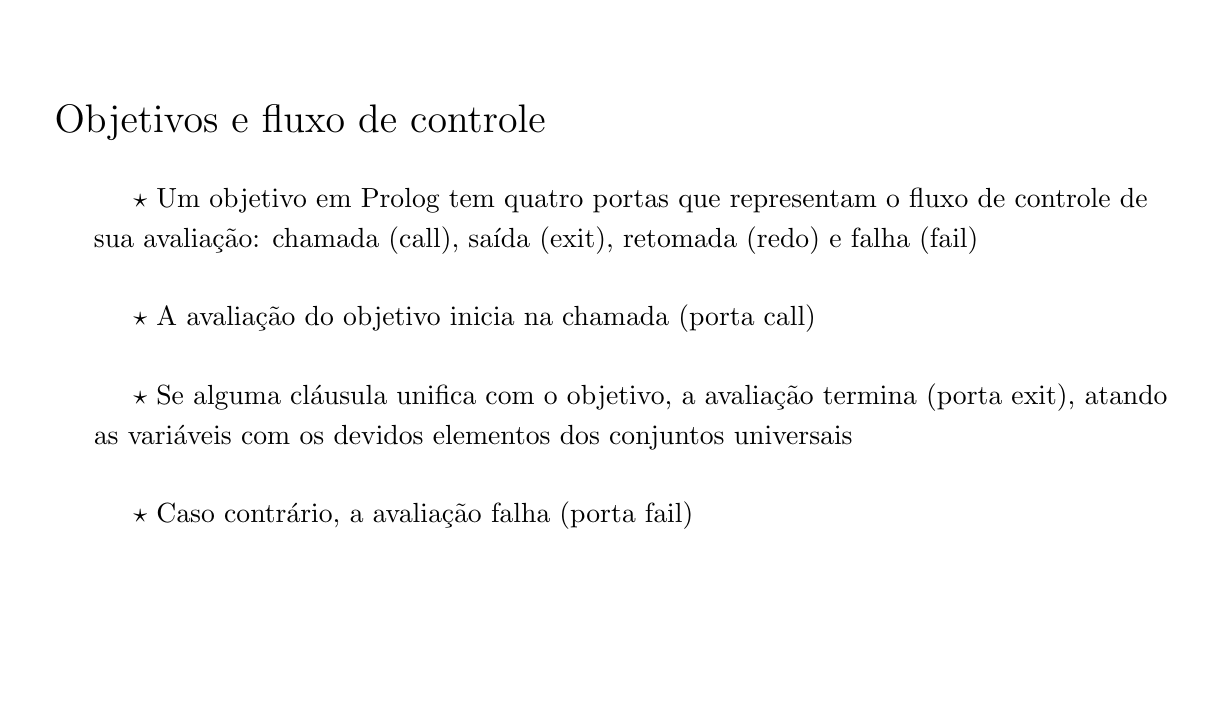
\begin{tikzpicture}
\node[draw,opacity=0] at (0, 0) {x};
\node[draw,opacity=0] at (14, 8) {x};

	\node[anchor=west] (title) at (0.0, 7.0) { \Large \bbbold{Objetivos e fluxo de controle} };


	\node[anchor=west] (a) at (1.0, 6.0) { $\star$ \bbtext{Um objetivo em Prolog tem quatro portas que representam o fluxo de controle de} };

	\node[anchor=west] (a1) at (0.5, 5.5) { \bbtext{sua avaliação: chamada (\bbenglish{call}), saída (\bbenglish{exit}), retomada (\bbenglish{redo}) e falha (\bbenglish{fail})} };


	\node[anchor=west] (b) at (1.0, 4.5) { $\star$ \bbtext{A avaliação do objetivo inicia na chamada (porta \bbenglish{call})} };

	\node[anchor=west] (c) at (1.0, 3.5) { $\star$ \bbtext{Se alguma cláusula unifica com o objetivo, a avaliação termina (porta \bbenglish{exit}), atando} };


	\node[anchor=west] (c1) at (0.5, 3.0) { \bbtext{as variáveis com os devidos elementos dos conjuntos universais} };

	\node[anchor=west] (d) at (1.0, 2.0) { $\star$ \bbtext{Caso contrário, a avaliação falha (porta \bbenglish{fail})} };

\end{tikzpicture}
\end{frame}
\begin{frame}[plain,t]
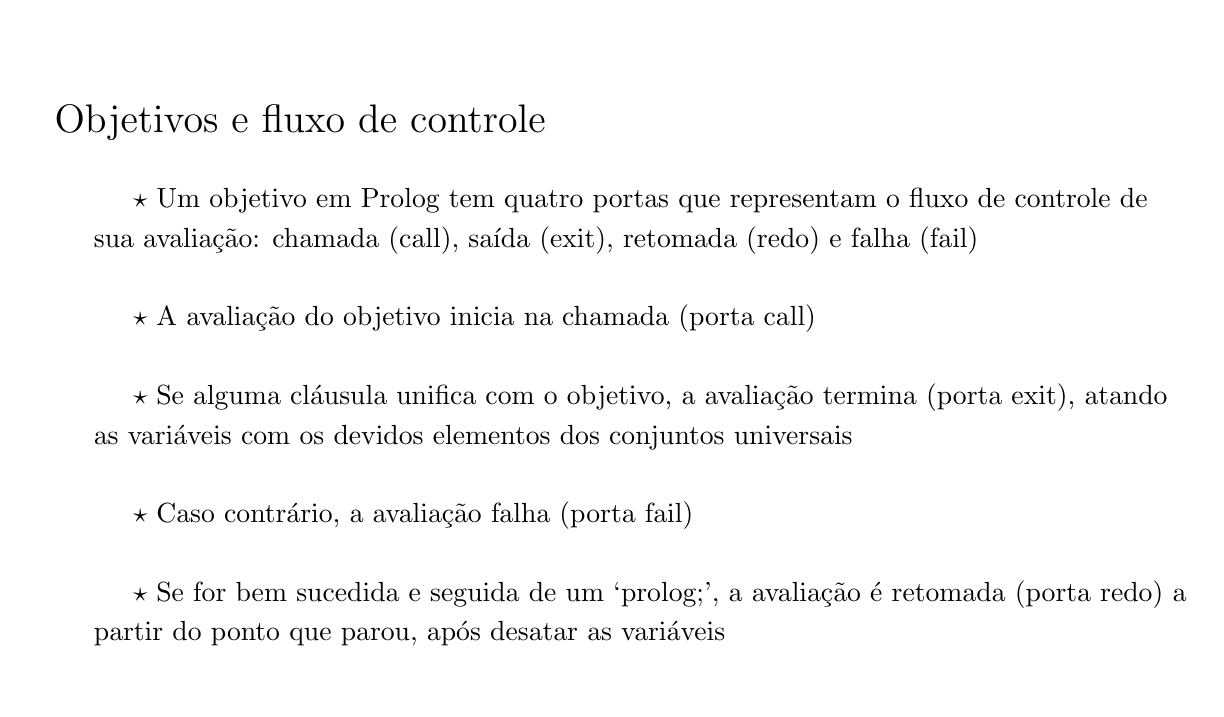
\begin{tikzpicture}
\node[draw,opacity=0] at (0, 0) {x};
\node[draw,opacity=0] at (14, 8) {x};

	\node[anchor=west] (title) at (0.0, 7.0) { \Large \bbbold{Objetivos e fluxo de controle} };


	\node[anchor=west] (a) at (1.0, 6.0) { $\star$ \bbtext{Um objetivo em Prolog tem quatro portas que representam o fluxo de controle de} };

	\node[anchor=west] (a1) at (0.5, 5.5) { \bbtext{sua avaliação: chamada (\bbenglish{call}), saída (\bbenglish{exit}), retomada (\bbenglish{redo}) e falha (\bbenglish{fail})} };


	\node[anchor=west] (b) at (1.0, 4.5) { $\star$ \bbtext{A avaliação do objetivo inicia na chamada (porta \bbenglish{call})} };

	\node[anchor=west] (c) at (1.0, 3.5) { $\star$ \bbtext{Se alguma cláusula unifica com o objetivo, a avaliação termina (porta \bbenglish{exit}), atando} };


	\node[anchor=west] (c1) at (0.5, 3.0) { \bbtext{as variáveis com os devidos elementos dos conjuntos universais} };

	\node[anchor=west] (d) at (1.0, 2.0) { $\star$ \bbtext{Caso contrário, a avaliação falha (porta \bbenglish{fail})} };

	\node[anchor=west] (e) at (1.0, 1.0) { $\star$ \bbtext{Se for bem sucedida e seguida de um `\code{prolog}{;}', a avaliação é retomada (porta \bbenglish{redo}) a} };


	\node[anchor=west] (e1) at (0.5, 0.5) { \bbtext{partir do ponto que parou, após desatar as variáveis} };

\end{tikzpicture}
\end{frame}
\begin{frame}[plain,t]
\begin{tikzpicture}
\node[draw,opacity=0] at (0, 0) {x};
\node[draw,opacity=0] at (14, 8) {x};

	\node[anchor=west] (title) at (0.0, 7.0) { \Large \bbbold{Visualização do fluxo de uma consulta simples em Prolog} };

	\draw[very thick] (4.5, 5.5) rectangle  (8.5, 1.5);

	\node[] (label) at (6.5, 3.5) { \bbtext{Objetivo} };

	\draw[color=BBViolet,thick,-latex] (3.5, 5.0) to  (4.5, 5.0);

	\node[anchor=east] (call) at (3.5, 5.05) { \bbenglish{call} };

	\draw[color=BBViolet,thick,latex-] (3.5, 2.0) to  (4.5, 2.0);

	\node[anchor=east] (fail) at (3.5, 2.0) { \bbenglish{fail} };

	\draw[color=BBViolet,thick,-latex] (8.5, 5.0) to  (9.5, 5.0);

	\node[anchor=west] (exit) at (9.5, 5.05) { \bbenglish{exit} };

	\draw[color=BBViolet,thick,latex-] (8.5, 2.0) to  (9.5, 2.0);

	\node[anchor=west] (redo) at (9.5, 2.05) { \bbenglish{redo} };

\end{tikzpicture}
\end{frame}
\begin{frame}[plain,t]
\begin{tikzpicture}
\node[draw,opacity=0] at (0, 0) {x};
\node[draw,opacity=0] at (14, 8) {x};

	\node[anchor=west] (title) at (0.0, 7.0) { \Large \bbbold{Consultas compostas} };

\end{tikzpicture}
\end{frame}
\begin{frame}[plain,t]
\begin{tikzpicture}
\node[draw,opacity=0] at (0, 0) {x};
\node[draw,opacity=0] at (14, 8) {x};

	\node[anchor=west] (title) at (0.0, 7.0) { \Large \bbbold{Consultas compostas} };


	\node[anchor=west] (a) at (1.0, 6.0) { $\star$ \bbtext{Consultas simples podem ser combinadas em consultas \bbbold{compostas} por meio do} };

	\node[anchor=west] (a1) at (0.5, 5.5) { \bbtext{operador `\code{prolog}{,/2}' (\bbbold{e} lógico)} };

\end{tikzpicture}
\end{frame}
\begin{frame}[plain,t]
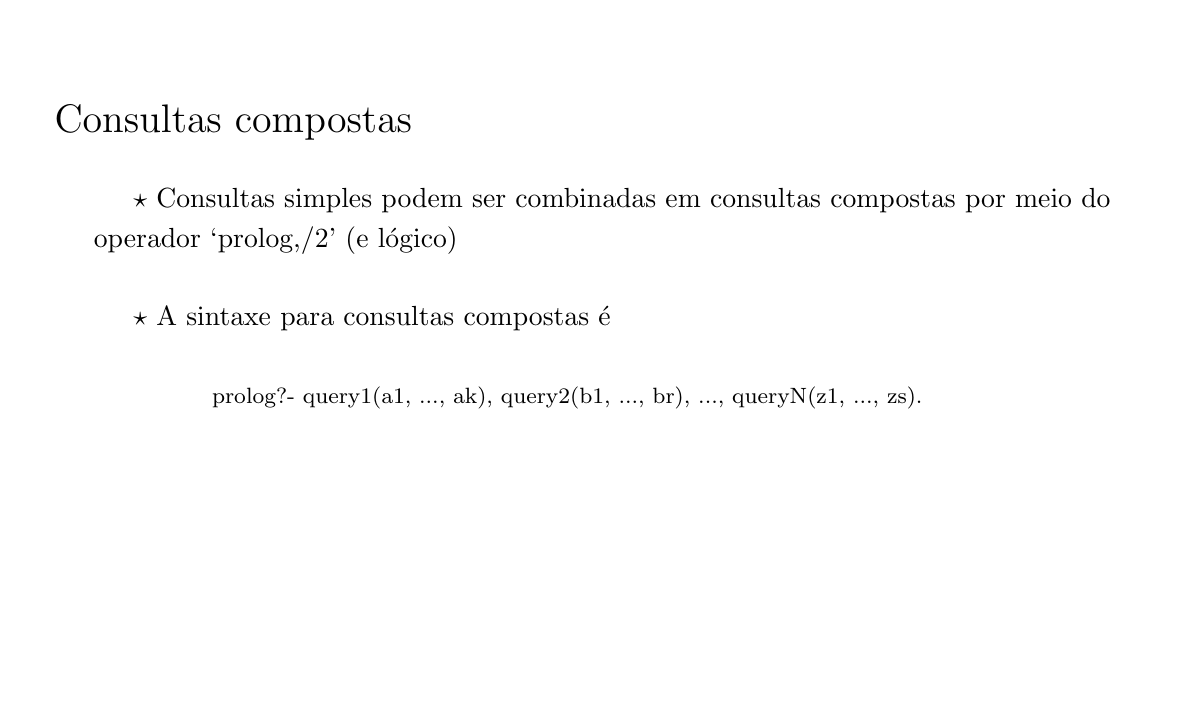
\begin{tikzpicture}
\node[draw,opacity=0] at (0, 0) {x};
\node[draw,opacity=0] at (14, 8) {x};

	\node[anchor=west] (title) at (0.0, 7.0) { \Large \bbbold{Consultas compostas} };


	\node[anchor=west] (a) at (1.0, 6.0) { $\star$ \bbtext{Consultas simples podem ser combinadas em consultas \bbbold{compostas} por meio do} };

	\node[anchor=west] (a1) at (0.5, 5.5) { \bbtext{operador `\code{prolog}{,/2}' (\bbbold{e} lógico)} };


	\node[anchor=west] (b) at (1.0, 4.5) { $\star$ \bbtext{A sintaxe para consultas compostas é} };

	\node[anchor=west] (b1) at (2.0, 3.5) { \footnotesize \code{prolog}{?- query1(a1, ..., ak), query2(b1, ..., br), ..., queryN(z1, ..., zs).} };

\end{tikzpicture}
\end{frame}
\begin{frame}[plain,t]
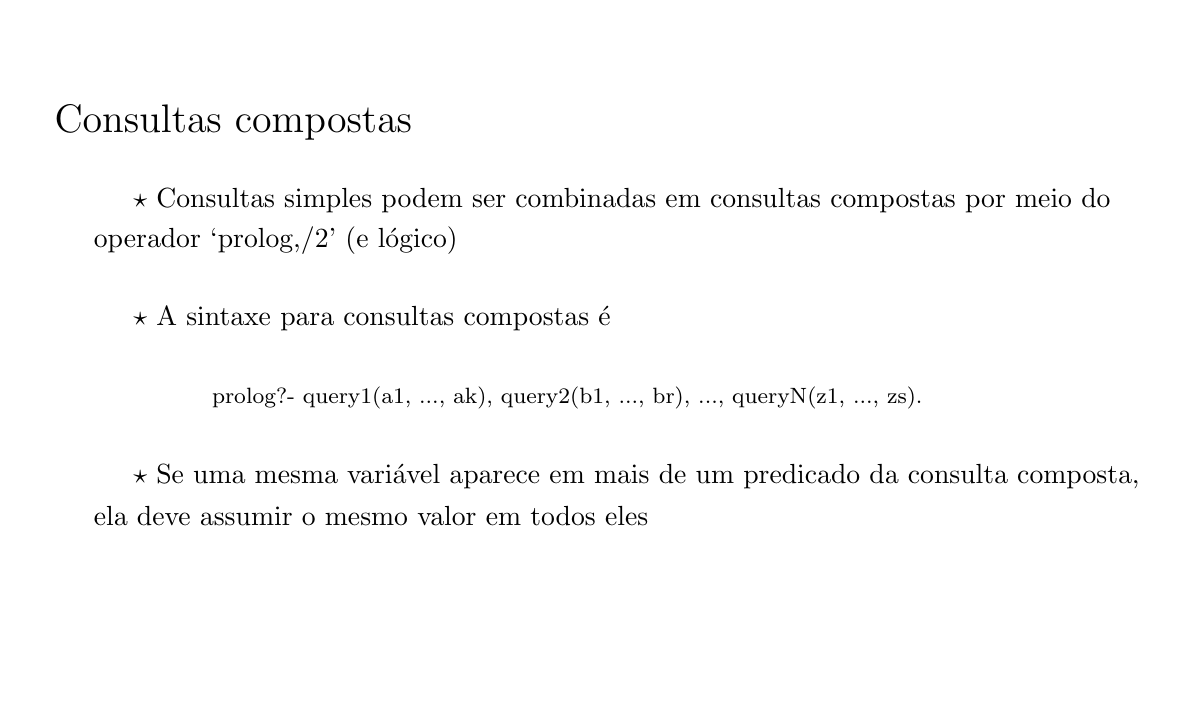
\begin{tikzpicture}
\node[draw,opacity=0] at (0, 0) {x};
\node[draw,opacity=0] at (14, 8) {x};

	\node[anchor=west] (title) at (0.0, 7.0) { \Large \bbbold{Consultas compostas} };


	\node[anchor=west] (a) at (1.0, 6.0) { $\star$ \bbtext{Consultas simples podem ser combinadas em consultas \bbbold{compostas} por meio do} };

	\node[anchor=west] (a1) at (0.5, 5.5) { \bbtext{operador `\code{prolog}{,/2}' (\bbbold{e} lógico)} };


	\node[anchor=west] (b) at (1.0, 4.5) { $\star$ \bbtext{A sintaxe para consultas compostas é} };

	\node[anchor=west] (b1) at (2.0, 3.5) { \footnotesize \code{prolog}{?- query1(a1, ..., ak), query2(b1, ..., br), ..., queryN(z1, ..., zs).} };


	\node[anchor=west] (c) at (1.0, 2.5) { $\star$ \bbtext{Se uma mesma variável aparece em mais de um predicado da consulta composta,} };

	\node[anchor=west] (c1) at (0.5, 2.0) { \bbtext{ela deve assumir o mesmo valor em todos eles} };

\end{tikzpicture}
\end{frame}
\begin{frame}[plain,t]
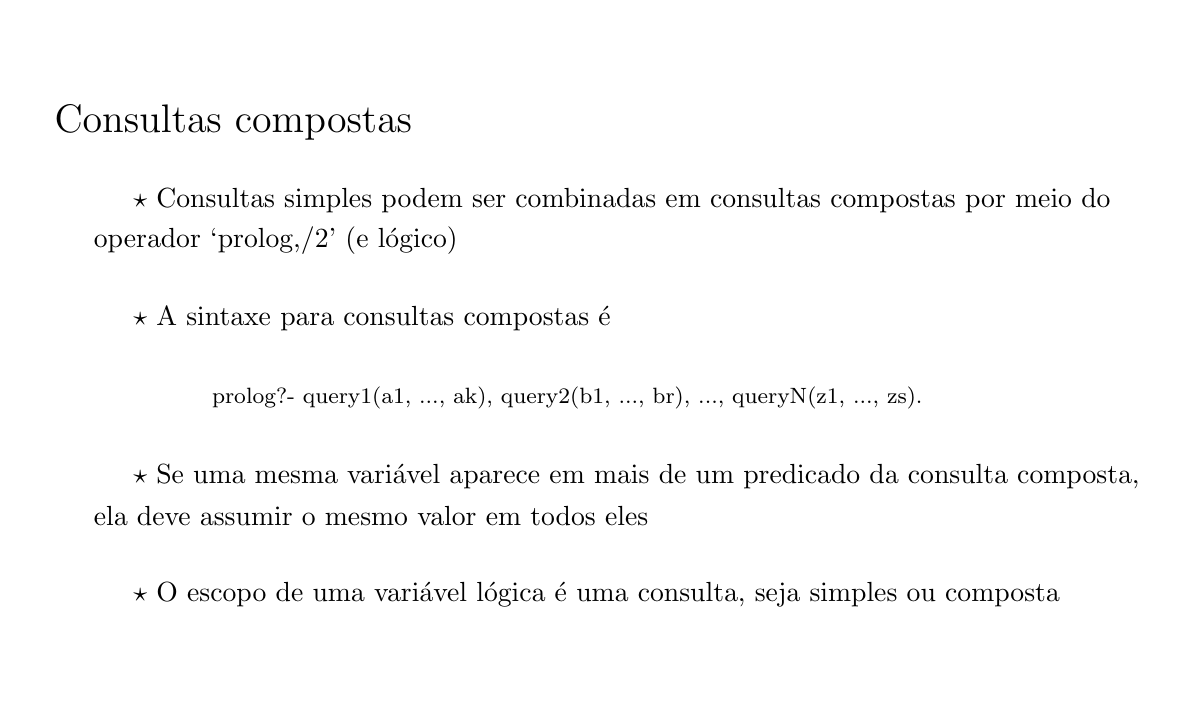
\begin{tikzpicture}
\node[draw,opacity=0] at (0, 0) {x};
\node[draw,opacity=0] at (14, 8) {x};

	\node[anchor=west] (title) at (0.0, 7.0) { \Large \bbbold{Consultas compostas} };


	\node[anchor=west] (a) at (1.0, 6.0) { $\star$ \bbtext{Consultas simples podem ser combinadas em consultas \bbbold{compostas} por meio do} };

	\node[anchor=west] (a1) at (0.5, 5.5) { \bbtext{operador `\code{prolog}{,/2}' (\bbbold{e} lógico)} };


	\node[anchor=west] (b) at (1.0, 4.5) { $\star$ \bbtext{A sintaxe para consultas compostas é} };

	\node[anchor=west] (b1) at (2.0, 3.5) { \footnotesize \code{prolog}{?- query1(a1, ..., ak), query2(b1, ..., br), ..., queryN(z1, ..., zs).} };


	\node[anchor=west] (c) at (1.0, 2.5) { $\star$ \bbtext{Se uma mesma variável aparece em mais de um predicado da consulta composta,} };

	\node[anchor=west] (c1) at (0.5, 2.0) { \bbtext{ela deve assumir o mesmo valor em todos eles} };


	\node[anchor=west] (d) at (1.0, 1.0) { $\star$ \bbtext{O escopo de uma variável lógica é uma consulta, seja simples ou composta} };

\end{tikzpicture}
\end{frame}
\begin{frame}[plain,t]
\begin{tikzpicture}
\node[draw,opacity=0] at (0, 0) {x};
\node[draw,opacity=0] at (14, 8) {x};

	\node[anchor=west] (title) at (0.0, 7.0) { \Large \bbbold{Fluxo de controle de consultas compostas} };

\end{tikzpicture}
\end{frame}
\begin{frame}[plain,t]
\begin{tikzpicture}
\node[draw,opacity=0] at (0, 0) {x};
\node[draw,opacity=0] at (14, 8) {x};

	\node[anchor=west] (title) at (0.0, 7.0) { \Large \bbbold{Fluxo de controle de consultas compostas} };

	\node[anchor=west] (a) at (1.0, 6.0) { $\star$ \bbtext{O \bbenglish{backtracking} tentar unificar todos os objetivos, da esquerda para a direita} };

\end{tikzpicture}
\end{frame}
\begin{frame}[plain,t]
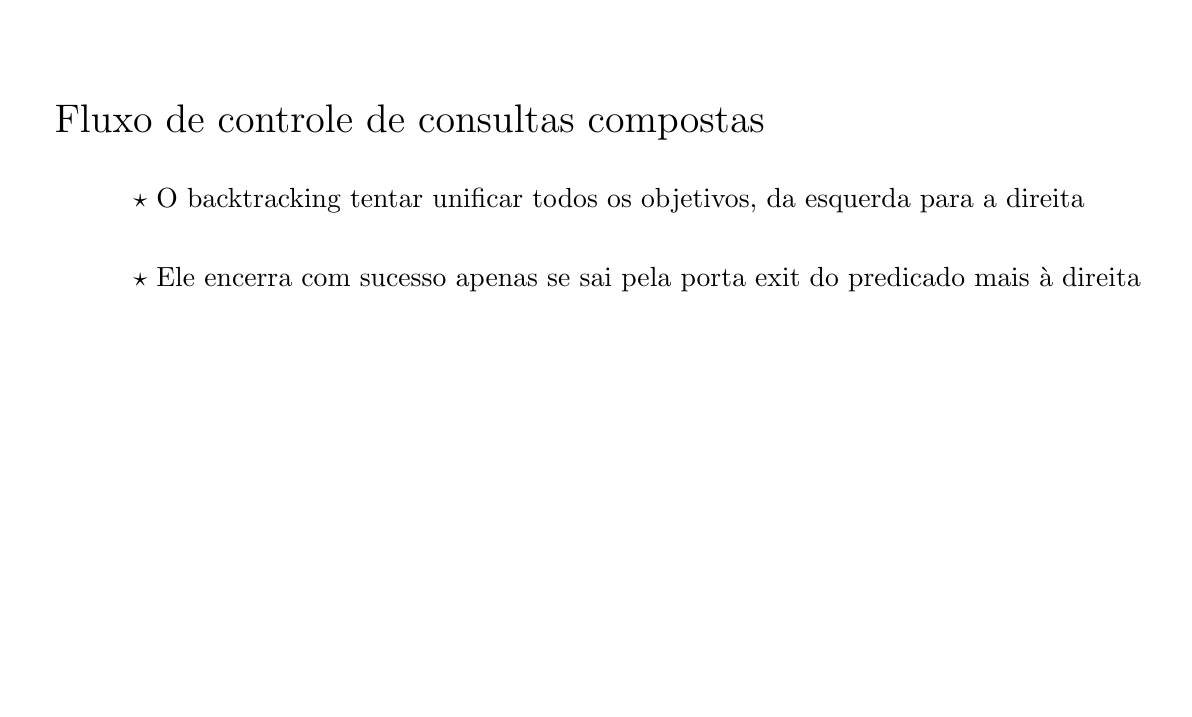
\begin{tikzpicture}
\node[draw,opacity=0] at (0, 0) {x};
\node[draw,opacity=0] at (14, 8) {x};

	\node[anchor=west] (title) at (0.0, 7.0) { \Large \bbbold{Fluxo de controle de consultas compostas} };

	\node[anchor=west] (a) at (1.0, 6.0) { $\star$ \bbtext{O \bbenglish{backtracking} tentar unificar todos os objetivos, da esquerda para a direita} };

	\node[anchor=west] (b) at (1.0, 5.0) { $\star$ \bbtext{Ele encerra com sucesso apenas se sai pela porta \bbenglish{exit} do predicado mais à direita} };


\end{tikzpicture}
\end{frame}
\begin{frame}[plain,t]
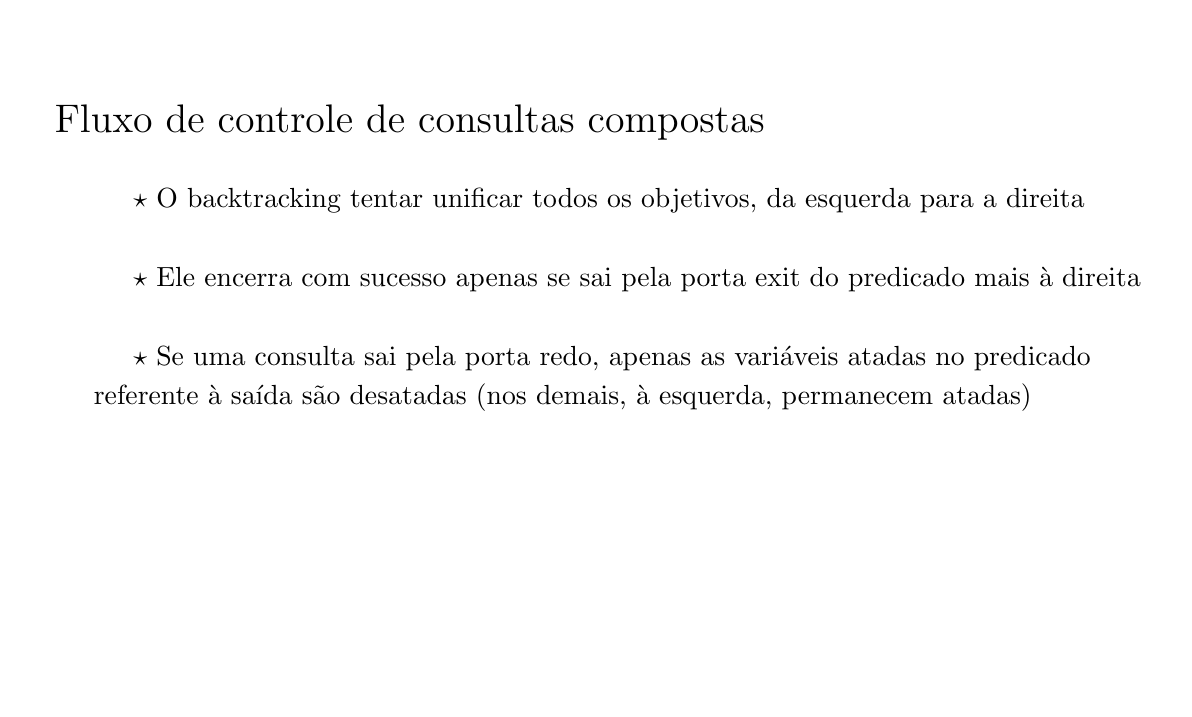
\begin{tikzpicture}
\node[draw,opacity=0] at (0, 0) {x};
\node[draw,opacity=0] at (14, 8) {x};

	\node[anchor=west] (title) at (0.0, 7.0) { \Large \bbbold{Fluxo de controle de consultas compostas} };

	\node[anchor=west] (a) at (1.0, 6.0) { $\star$ \bbtext{O \bbenglish{backtracking} tentar unificar todos os objetivos, da esquerda para a direita} };

	\node[anchor=west] (b) at (1.0, 5.0) { $\star$ \bbtext{Ele encerra com sucesso apenas se sai pela porta \bbenglish{exit} do predicado mais à direita} };


	\node[anchor=west] (c) at (1.0, 4.0) { $\star$ \bbtext{Se uma consulta sai pela porta \bbenglish{redo}, apenas as variáveis atadas no predicado} };


	\node[anchor=west] (c1) at (0.5, 3.5) { \bbtext{referente à saída são desatadas (nos demais, à esquerda, permanecem atadas)} };

\end{tikzpicture}
\end{frame}
\begin{frame}[plain,t]
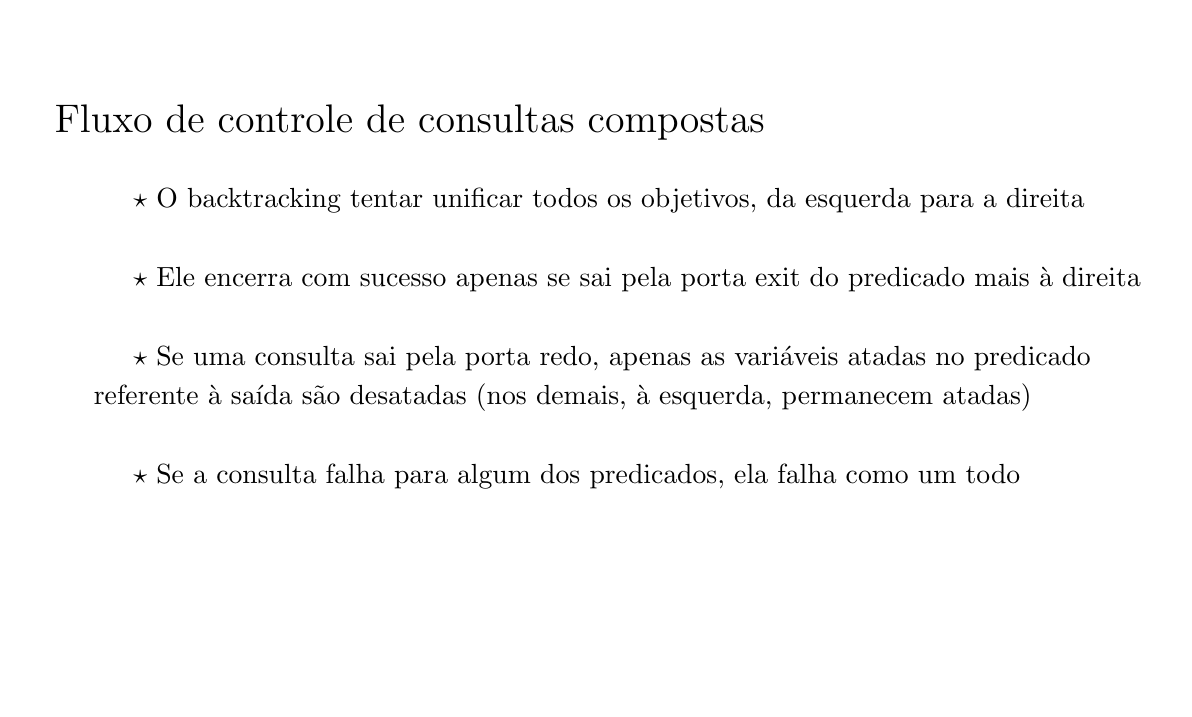
\begin{tikzpicture}
\node[draw,opacity=0] at (0, 0) {x};
\node[draw,opacity=0] at (14, 8) {x};

	\node[anchor=west] (title) at (0.0, 7.0) { \Large \bbbold{Fluxo de controle de consultas compostas} };

	\node[anchor=west] (a) at (1.0, 6.0) { $\star$ \bbtext{O \bbenglish{backtracking} tentar unificar todos os objetivos, da esquerda para a direita} };

	\node[anchor=west] (b) at (1.0, 5.0) { $\star$ \bbtext{Ele encerra com sucesso apenas se sai pela porta \bbenglish{exit} do predicado mais à direita} };


	\node[anchor=west] (c) at (1.0, 4.0) { $\star$ \bbtext{Se uma consulta sai pela porta \bbenglish{redo}, apenas as variáveis atadas no predicado} };


	\node[anchor=west] (c1) at (0.5, 3.5) { \bbtext{referente à saída são desatadas (nos demais, à esquerda, permanecem atadas)} };

	\node[anchor=west] (d) at (1.0, 2.5) { $\star$ \bbtext{Se a consulta falha para algum dos predicados, ela falha como um todo} };

\end{tikzpicture}
\end{frame}
\begin{frame}[plain,t]
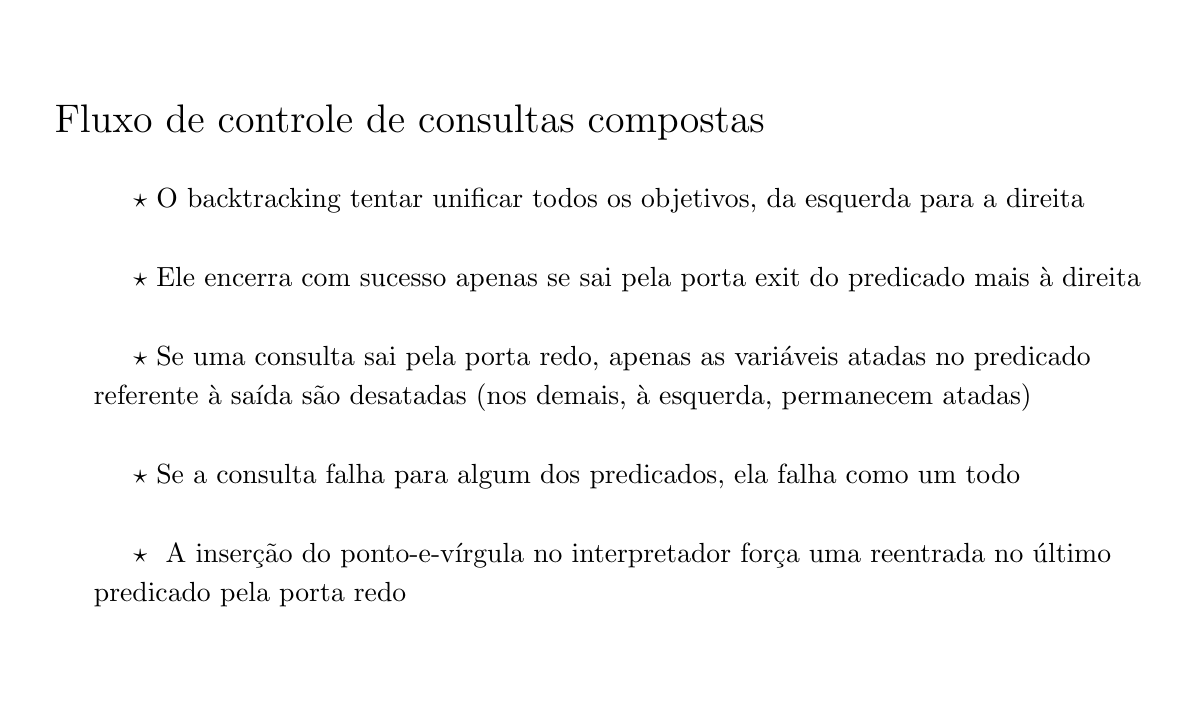
\begin{tikzpicture}
\node[draw,opacity=0] at (0, 0) {x};
\node[draw,opacity=0] at (14, 8) {x};

	\node[anchor=west] (title) at (0.0, 7.0) { \Large \bbbold{Fluxo de controle de consultas compostas} };

	\node[anchor=west] (a) at (1.0, 6.0) { $\star$ \bbtext{O \bbenglish{backtracking} tentar unificar todos os objetivos, da esquerda para a direita} };

	\node[anchor=west] (b) at (1.0, 5.0) { $\star$ \bbtext{Ele encerra com sucesso apenas se sai pela porta \bbenglish{exit} do predicado mais à direita} };


	\node[anchor=west] (c) at (1.0, 4.0) { $\star$ \bbtext{Se uma consulta sai pela porta \bbenglish{redo}, apenas as variáveis atadas no predicado} };


	\node[anchor=west] (c1) at (0.5, 3.5) { \bbtext{referente à saída são desatadas (nos demais, à esquerda, permanecem atadas)} };

	\node[anchor=west] (d) at (1.0, 2.5) { $\star$ \bbtext{Se a consulta falha para algum dos predicados, ela falha como um todo} };

	\node[anchor=west] (e) at (1.0, 1.5) { $\star$ \bbtext{ A inserção do ponto-e-vírgula no interpretador força uma reentrada no último} };

	\node[anchor=west] (e1) at (0.5, 1.0) { \bbtext{predicado pela porta \bbenglish{redo}} };

\end{tikzpicture}
\end{frame}
\begin{frame}[plain,t]
\begin{tikzpicture}
\node[draw,opacity=0] at (0, 0) {x};
\node[draw,opacity=0] at (14, 8) {x};

	\node[anchor=west] (title) at (0.0, 7.0) { \Large \bbbold{Visualização do fluxo de uma consulta composta em Prolog} };

	\draw[very thick] (1.5, 5.0) rectangle  (4.5, 2.0);

	\draw[very thick] (5.5, 5.0) rectangle  (8.5, 2.0);

	\draw[very thick] (9.5, 5.0) rectangle  (12.5, 2.0);


	\node[] (label1) at (3.0, 3.5) { \LARGE $Q_1$ };

	\node[] (label2) at (7.0, 3.5) { \LARGE $Q_2$ };

	\node[] (label3) at (11.0, 3.5) { \LARGE $Q_3$ };


	\draw[color=BBViolet,thick,-latex] (0.5, 4.5) to  (1.5, 4.5);

	\draw[color=BBViolet,thick,-latex] (4.5, 4.5) to  (5.5, 4.5);

	\draw[color=BBViolet,thick,-latex] (8.5, 4.5) to  (9.5, 4.5);


	\node[anchor=east] (call) at (0.5, 4.5) { \bbenglish{call} };

	\draw[color=BBViolet,thick,latex-] (0.5, 2.5) to  (1.5, 2.5);

	\draw[color=BBViolet,thick,latex-] (4.5, 2.5) to  (5.5, 2.5);

	\draw[color=BBViolet,thick,latex-] (8.5, 2.5) to  (9.5, 2.5);


	\node[anchor=east] (fail) at (0.5, 2.5) { \bbenglish{fail} };

	\draw[color=BBViolet,thick,-latex] (12.5, 4.5) to  (13.5, 4.5);

	\node[anchor=west] (exit) at (13.5, 4.5) { \bbenglish{exit} };

	\draw[color=BBViolet,thick,latex-] (12.5, 2.5) to  (13.5, 2.5);

	\node[anchor=west] (redo) at (13.5, 2.5) { \bbenglish{redo} };

\end{tikzpicture}
\end{frame}
\begin{frame}[plain,t]
\vspace*{\fill}

\inputsnippet{prolog}{1}{17}{codes/capital.pl}

\vspace*{\fill}
\end{frame}
\end{document}
